=========================================================% CAPÍTULO 4 — RESULTADOS Y ANÁLISIS% =========================================================

\chapter{Resultados y Análisis}
\label{cap}

% =========================================================
\section{Evolución del polvo}
\label{sec:Evolución_de_polvo}
% =========================================================

Esta sección analiza cómo la evolución del polvo responde a tres parámetros físicos
que controlan el transporte de sólidos en discos protoplanetarios estructurados:
la velocidad de fragmentación $v_{\rm frag}$, la intensidad de las perturbaciones
de presión y el nivel de turbulencia parametrizado mediante $\alpha$. La evolución
se estudia a partir de diagramas de Hovmöller de la relación polvo-gas
$\Sigma_d/\Sigma_g$, comparando discos suaves con discos que contienen una única
trampa de presión o una estructura sinusoidal de múltiples anillos.

% =========================================================
\invisiblesubsection{Impacto de la Velocidad de Fragmentación}
% =========================================================

La Figura~\ref{fig:hovmoller_vfrag} muestra la evolución espacio-temporal de
$\Sigma_d/\Sigma_g$ para tres velocidades de fragmentación
($v_{\rm frag}=1,\;3,\;10\,{\rm m\,s^{-1}}$), manteniendo fijo
$\alpha=10^{-3}$ y considerando tres arquitecturas del disco:
suave, gap único y perfil sinusoidal.

\begin{figure}[h!]
    \centering
    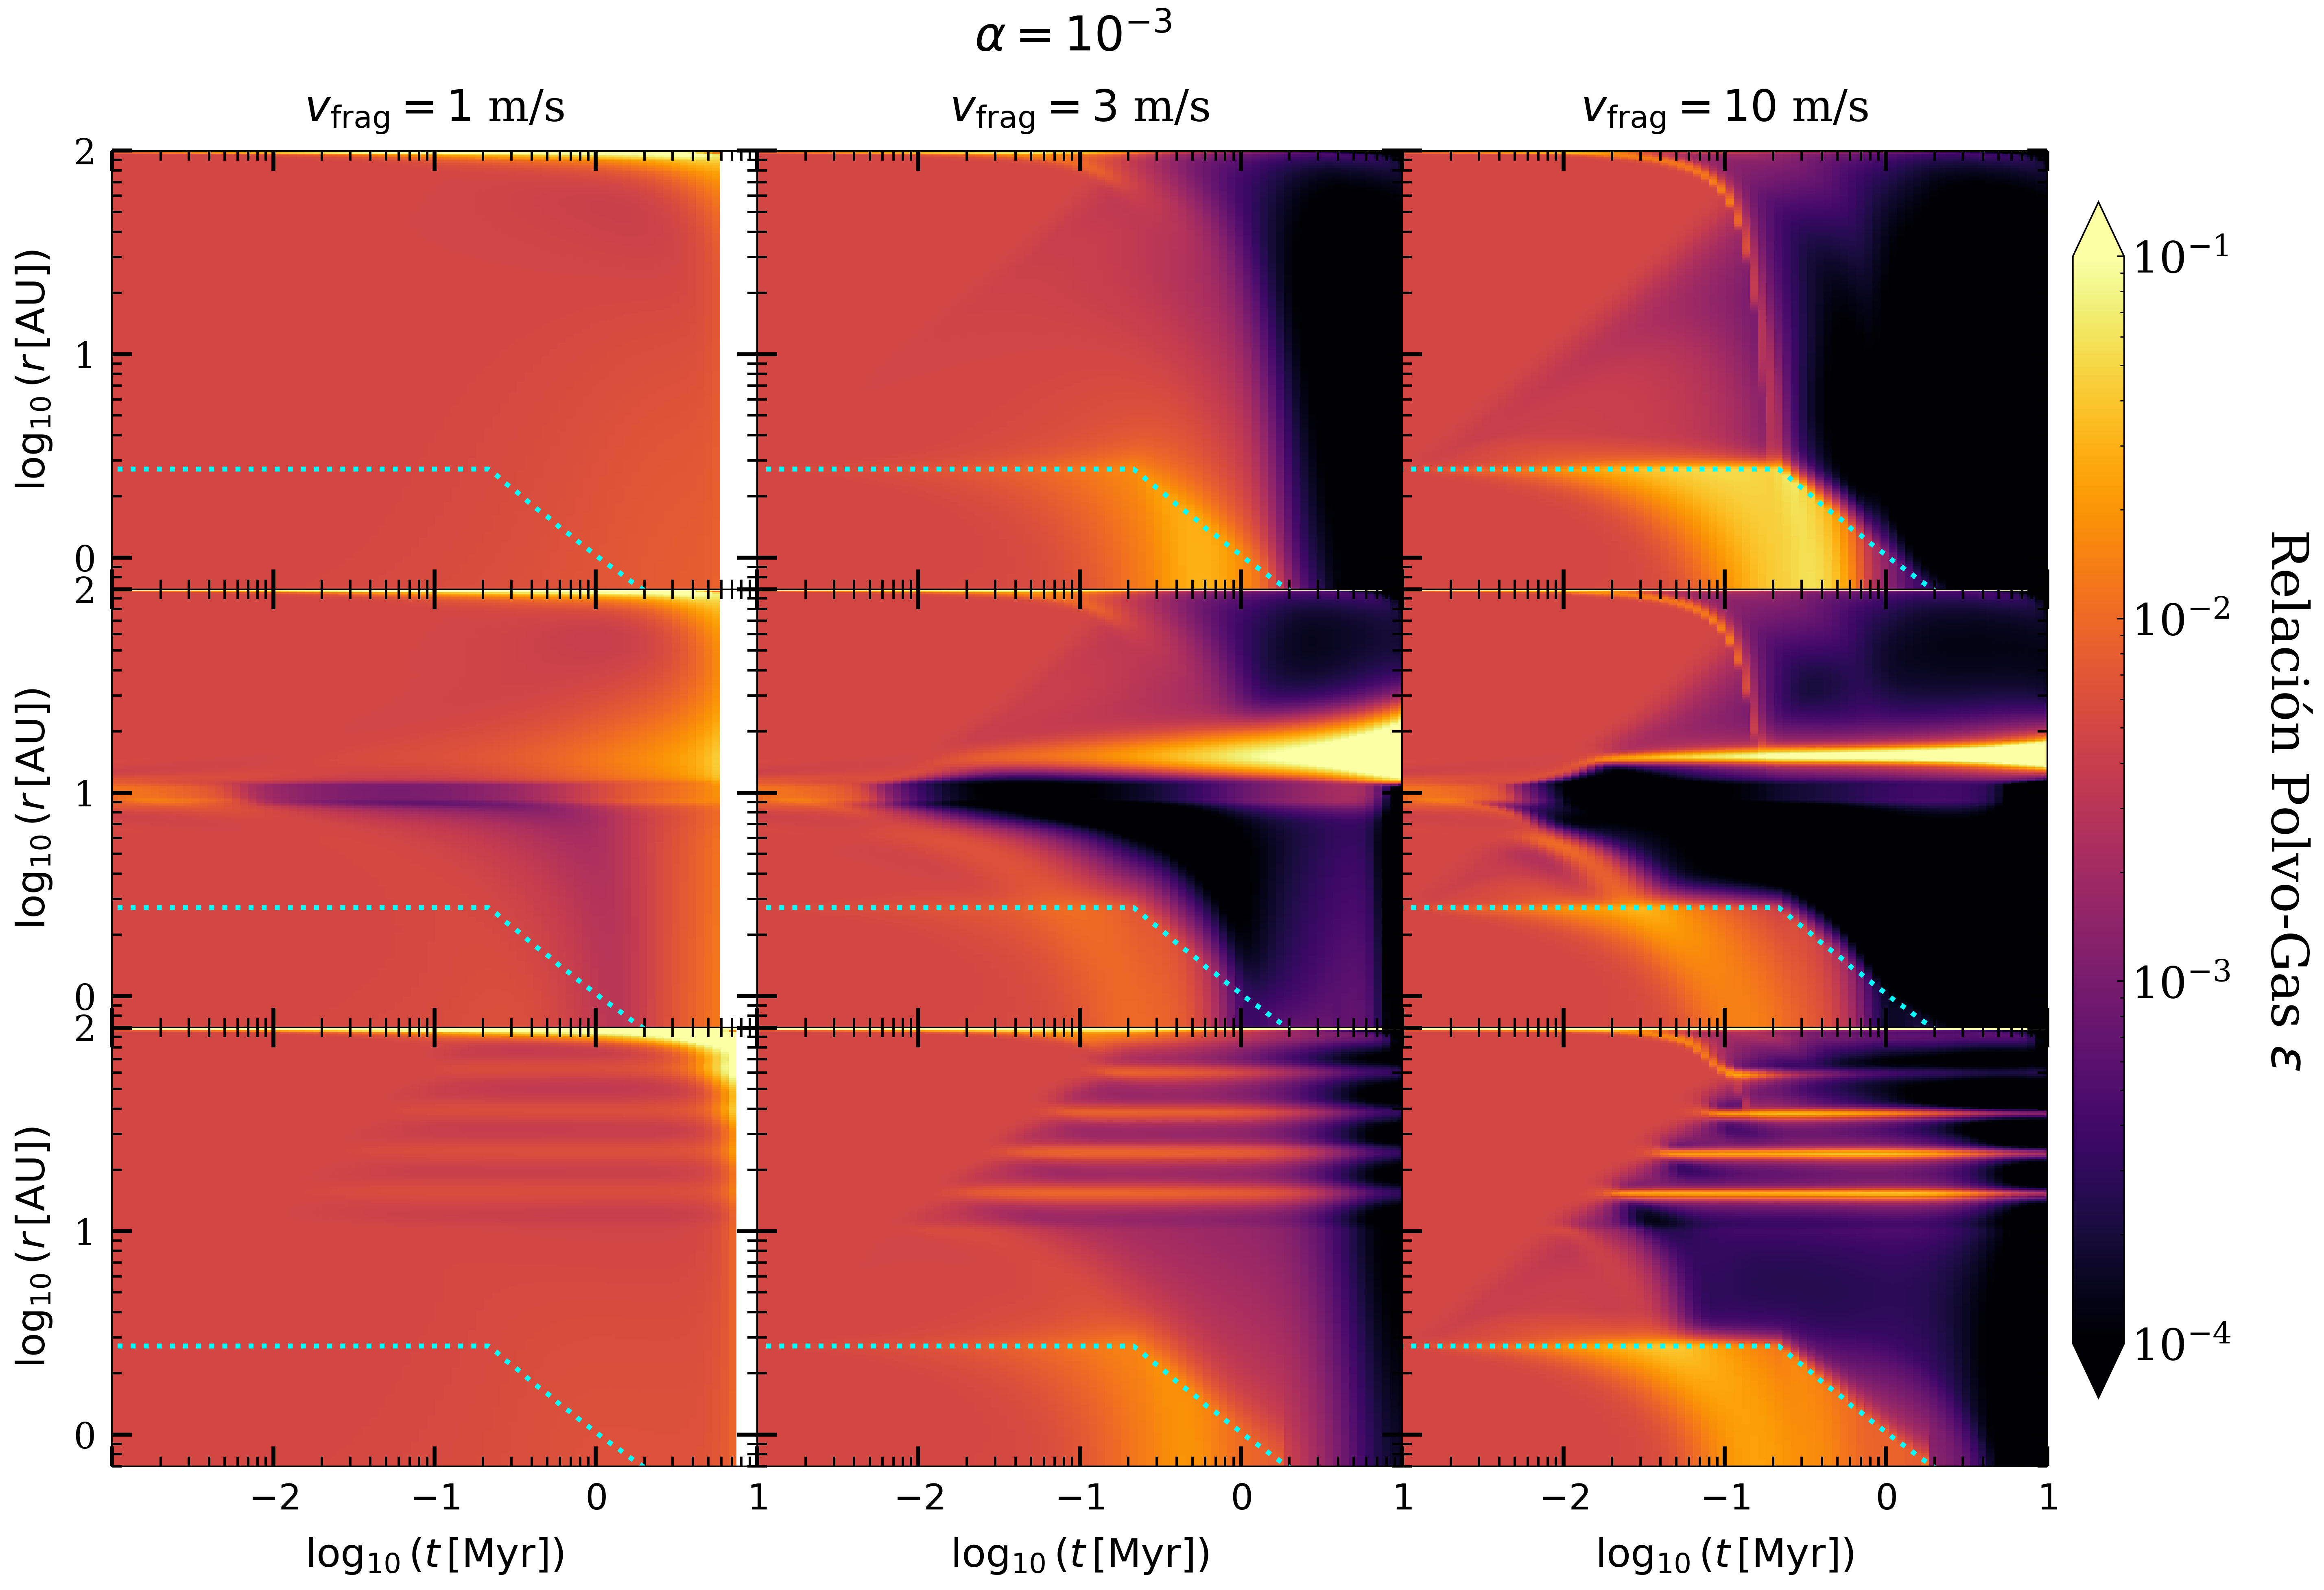
\includegraphics[width=\textwidth]{figures/4_fig_resultados/figura1_vfrags.png}
    \caption{Diagramas de Hovmöller de $\Sigma_d/\Sigma_g$ para
    $v_{\rm frag}=1,\;3,\;10\,{\rm m\,s^{-1}}$ (columnas) y tres arquitecturas
    del disco (filas): disco suave, gap único y perfil sinusoidal.
    La línea cian punteada indica la posición temporal del snowline.}
    \label{fig:hovmoller_vfrag}
\end{figure}

En el disco suave, la distribución de polvo evoluciona de manera similar para los
tres valores de $v_{\rm frag}$. La relación polvo-gas disminuye progresivamente
hacia radios pequeños debido a la deriva radial, sin observarse acumulaciones
locales persistentes. En ausencia de máximos de presión, modificar la velocidad
de fragmentación tiene un efecto reducido sobre la distribución global del polvo.

La situación cambia al introducir subestructuras. Tanto en el disco con un único
gap como en el perfil sinusoidal, el incremento de $v_{\rm frag}$ favorece la
formación de anillos con mayor relación polvo-gas. Para
$v_{\rm frag}=1\,{\rm m\,s^{-1}}$ la acumulación es prácticamente inexistente,
mientras que para $v_{\rm frag}=10\,{\rm m\,s^{-1}}$ aparecen reservorios sólidos
bien definidos en los máximos locales de presión.

Cuando el snowline alcanza estas regiones de acumulación
($t\sim1\,{\rm Myr}$), el comportamiento también depende de
$v_{\rm frag}$. En el caso de alta velocidad de fragmentación se observa la
liberación del material previamente retenido, visible como un aumento transitorio
de $\Sigma_d/\Sigma_g$ en el disco interior. Este fenómeno no aparece de forma
apreciable para $v_{\rm frag}=1\,{\rm m\,s^{-1}}$, donde la ausencia de un
reservorio sólido impide un transporte posterior de material hacia radios menores.

En conjunto, estos resultados muestran que el efecto de $v_{\rm frag}$ se manifiesta
principalmente cuando existen trampas de presión capaces de almacenar material.
En discos sin subestructuras, la evolución continúa dominada por la deriva radial.

% =========================================================
\invisiblesubsection{Dependencia con la Amplitud de la Perturbación}
% =========================================================

La Figura~\ref{fig:hovmoller_arquitectura} muestra la evolución del polvo al variar
la intensidad de la perturbación, representada por la masa del planeta que abre el
gap o por la amplitud del perfil sinusoidal, manteniendo
$v_{\rm frag}=10\,{\rm m\,s^{-1}}$ y $\alpha=10^{-3}$.

\begin{figure}[H]
    \centering
    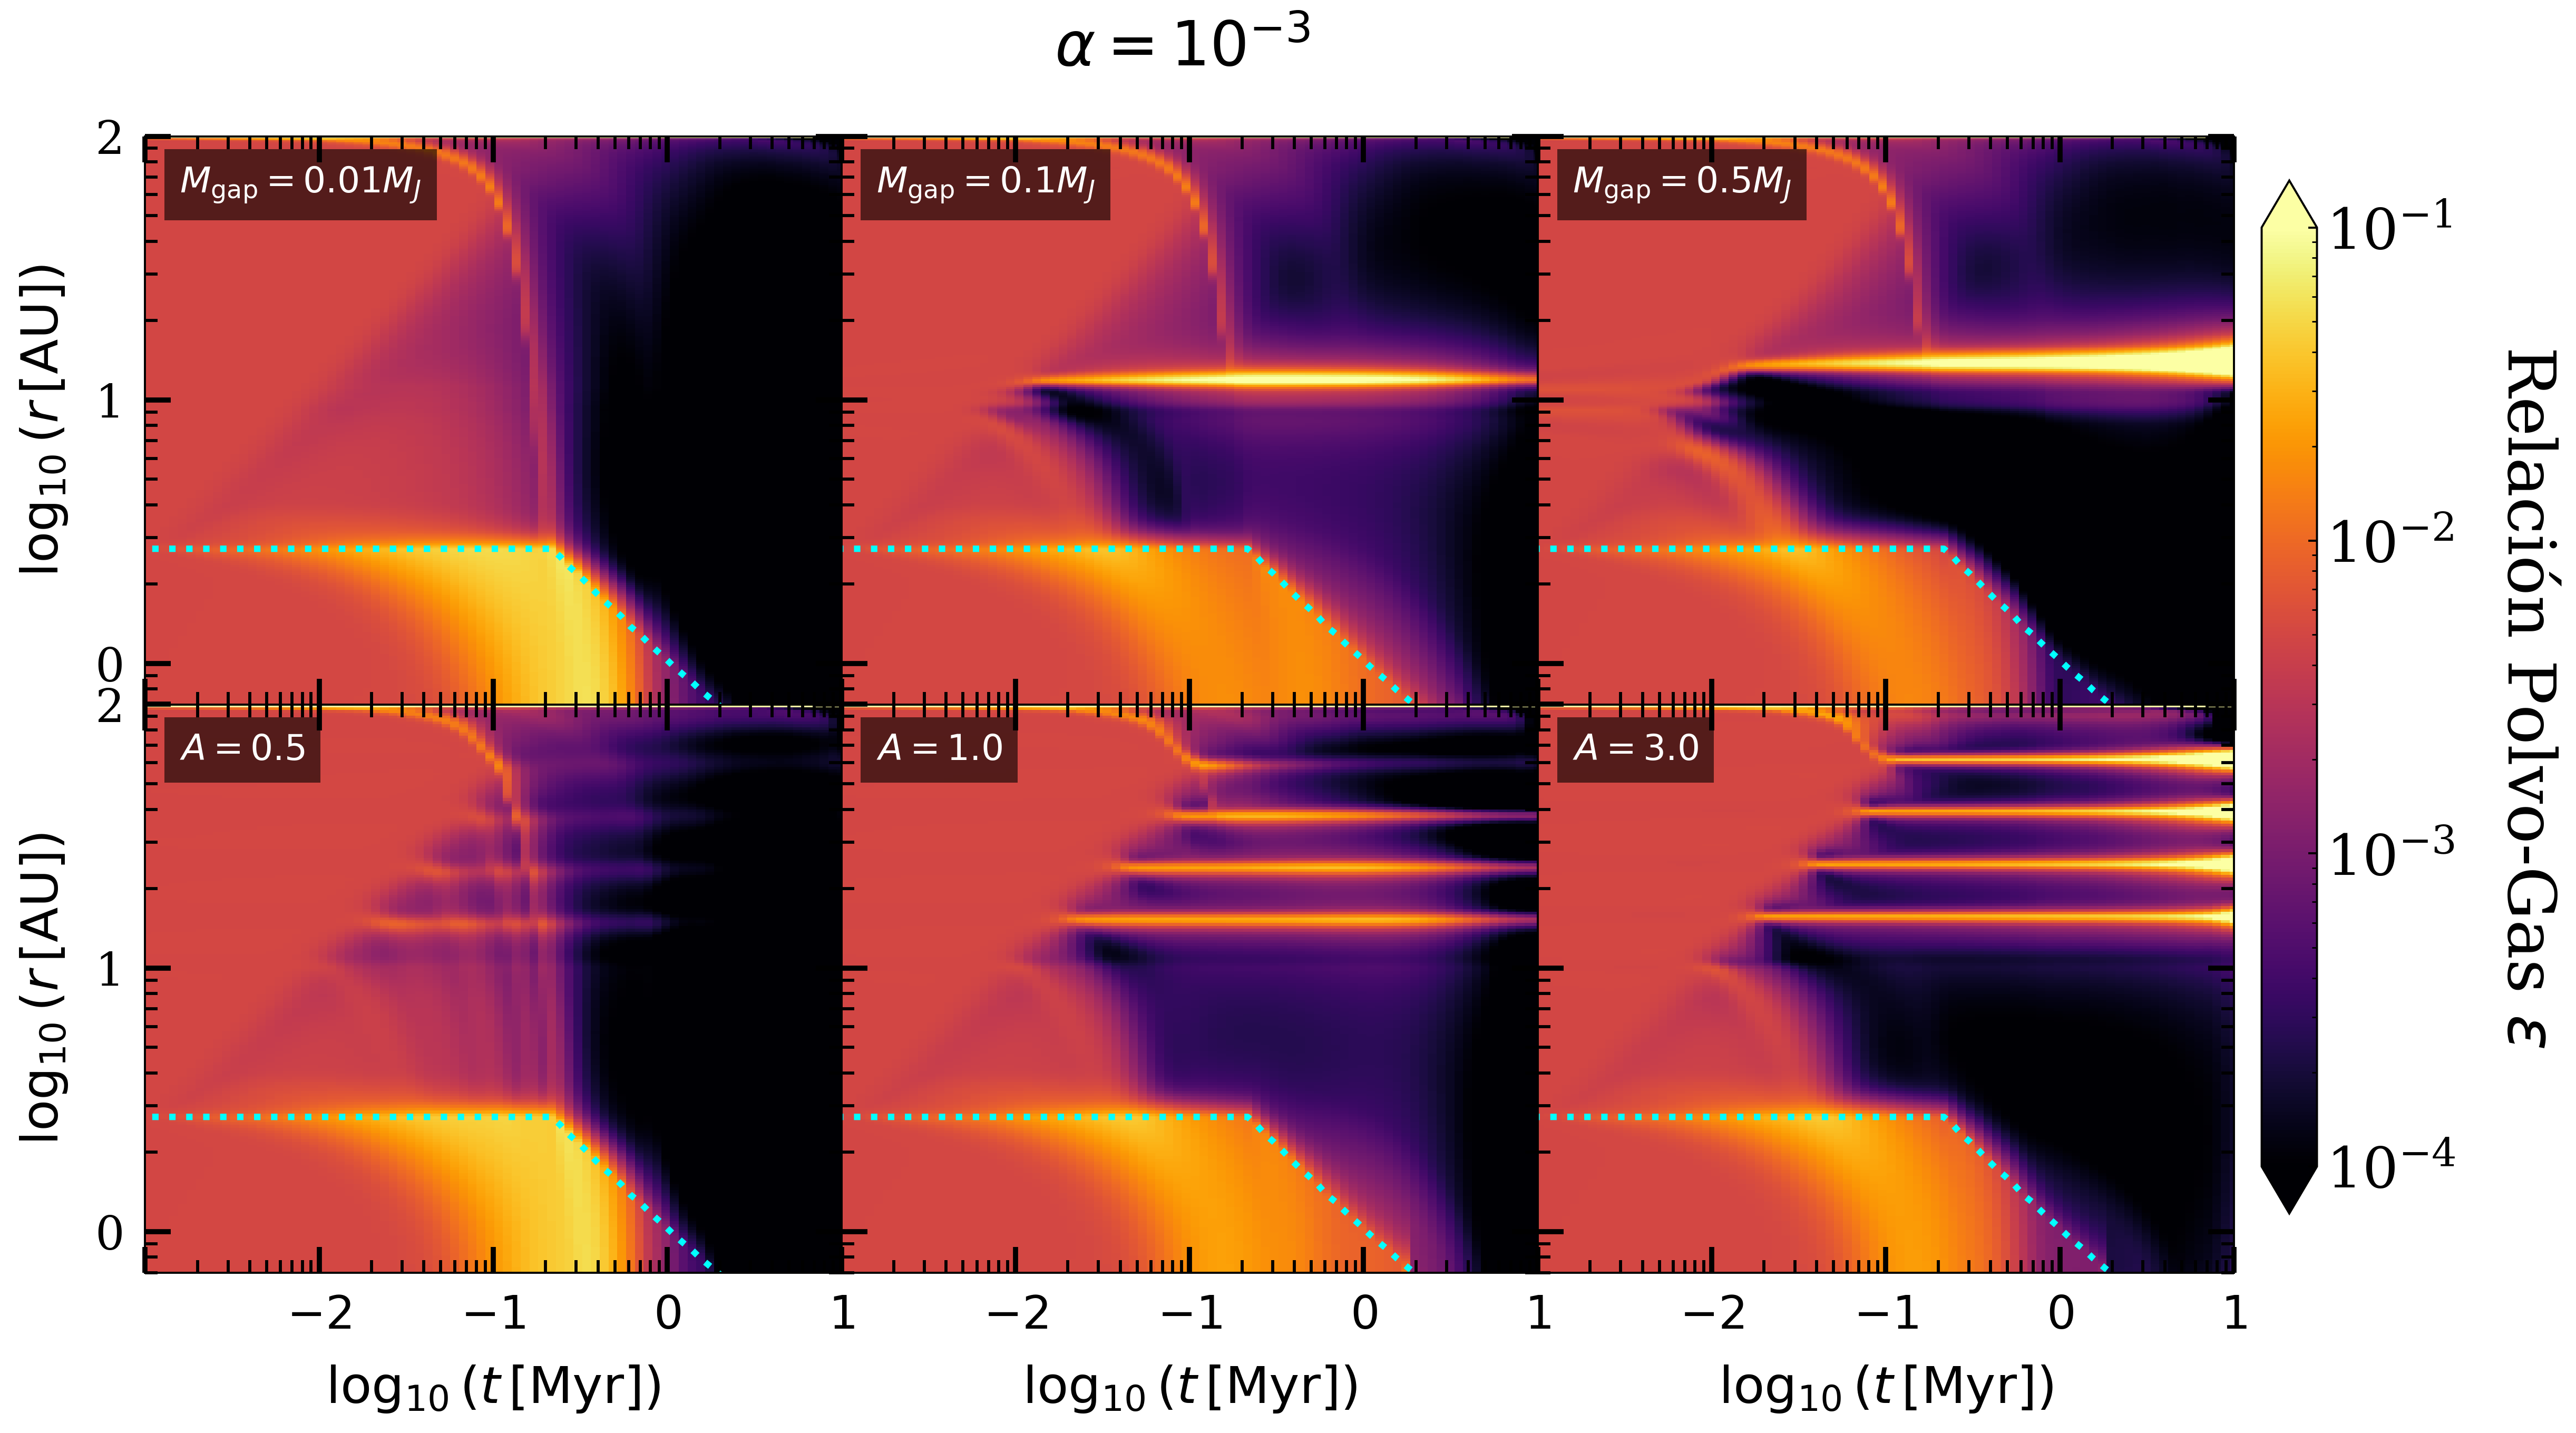
\includegraphics[width=1\textwidth]{figures/4_fig_resultados/figura2_masas.png}
    \caption{Diagramas de Hovmöller variando la amplitud de la perturbación para
    $v_{\rm frag}=10\,{\rm m\,s^{-1}}$ y $\alpha=10^{-3}$.}
    \label{fig:hovmoller_arquitectura}
\end{figure}

Para perturbaciones débiles
($M_{\rm gap}=0.01\,M_{\rm Jup}$ o $A=0.5$), la estructura de presión resulta
insuficiente para generar una acumulación significativa de sólidos. La relación
polvo-gas permanece cercana a la del disco suave durante toda la evolución.

Al aumentar la amplitud de la perturbación
($M_{\rm gap}=0.1\,M_{\rm Jup}$ o $A=1.0$), se desarrolla un anillo bien definido
con relaciones polvo-gas del orden de $10^{-2}$--$10^{-1}$. Cuando el snowline
atraviesa esta región, parte del material retenido es transportado nuevamente hacia
el disco interior, produciendo un episodio transitorio de enriquecimiento en polvo.

En el régimen de perturbaciones más intensas
($M_{\rm gap}=0.5\,M_{\rm Jup}$ o $A=3.0$), la acumulación inicial es aún mayor,
pero el reservorio permanece estable durante el resto de la evolución. Incluso
después del cruce del snowline, la mayor parte del material continúa retenida en
el borde exterior de la trampa, manteniendo empobrecidas las regiones interiores.

En conjunto, estos resultados muestran que la eficiencia del atrapamiento de polvo depende de manera no monótona de la intensidad de la perturbación. Mientras perturbaciones débiles no generan reservorios significativos, perturbaciones excesivamente profundas retienen el material durante toda la evolución del disco, limitando su liberación posterior hacia las regiones internas.

% =========================================================
\invisiblesubsection{Efecto de la Turbulencia}
% =========================================================

La Figura~\ref{fig:hovmoller_turbulencia} presenta la evolución del polvo para
$\alpha=10^{-4}$, $5\times10^{-4}$ y $10^{-3}$, utilizando
$v_{\rm frag}=10\,{\rm m\,s^{-1}}$ y la configuración de perturbación que produce
la acumulación más eficiente en la sección anterior.

\begin{figure}[H]
    \centering
    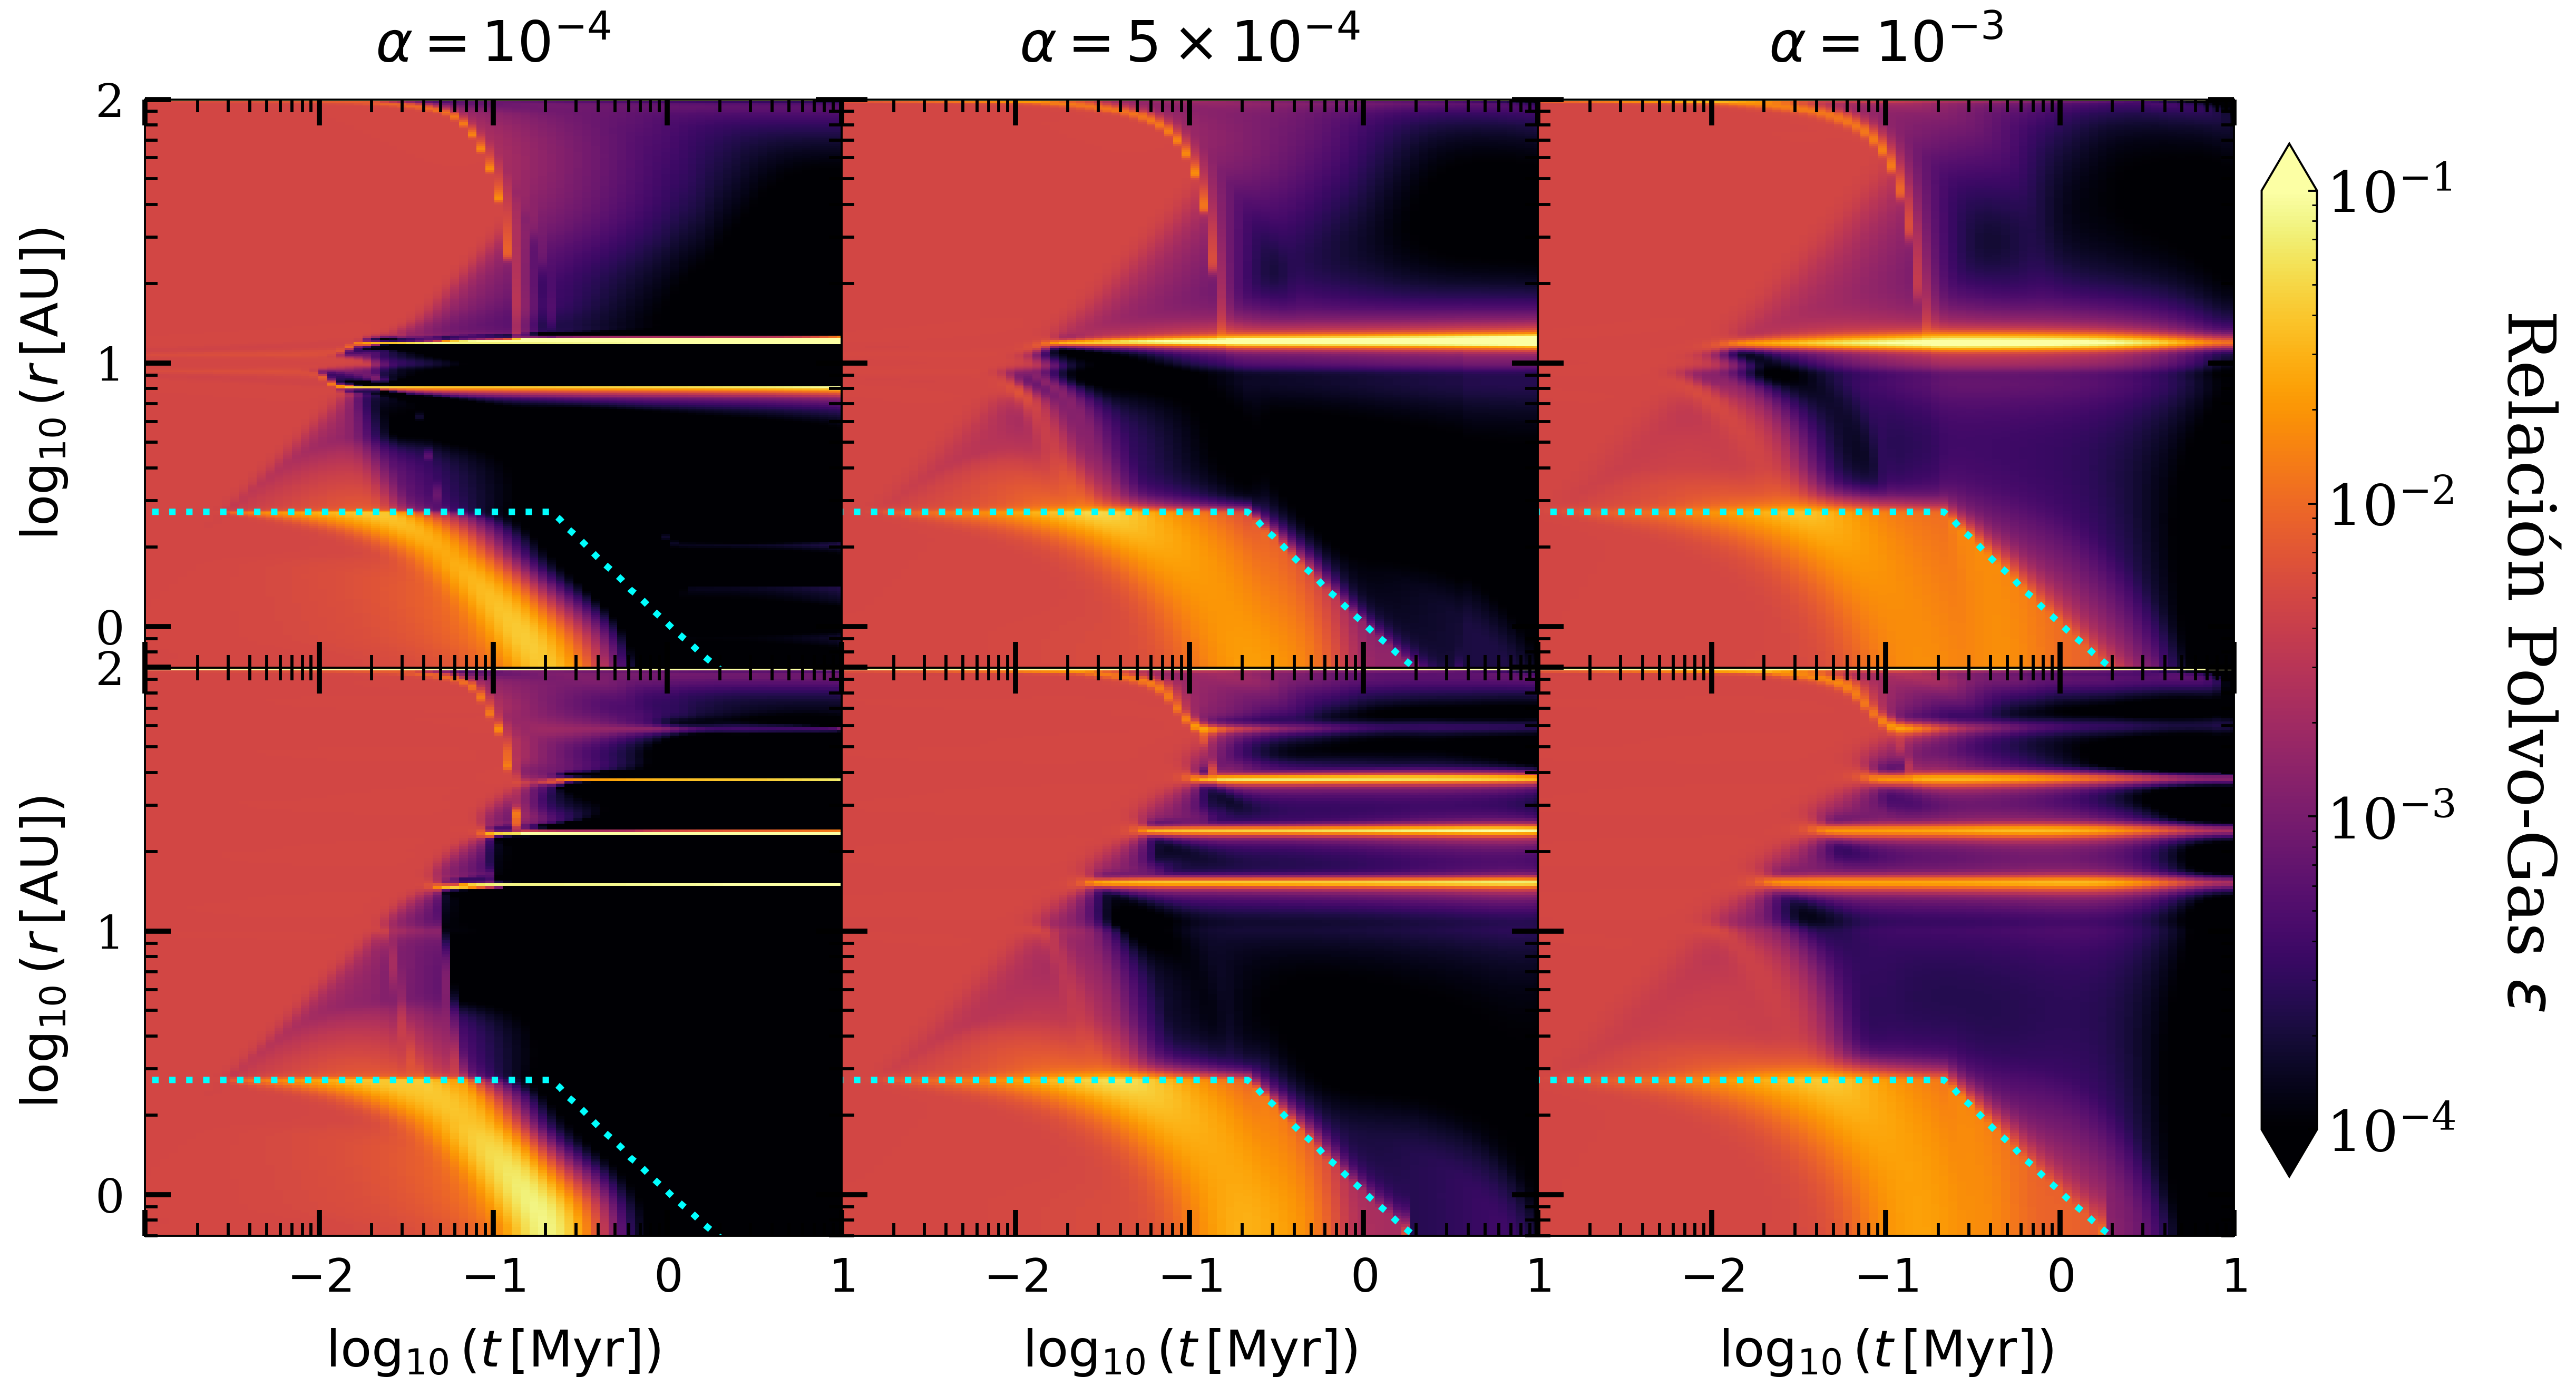
\includegraphics[width=\textwidth]{figures/4_fig_resultados/figura3_turbulencia.png}
    \caption{Diagramas de Hovmöller variando el parámetro turbulento $\alpha$.}
    \label{fig:hovmoller_turbulencia}
\end{figure}

Para $\alpha=10^{-4}$ se desarrollan anillos estrechos y con elevada concentración
de polvo, alcanzando relaciones $\Sigma_d/\Sigma_g$ cercanas a $10^{-1}$ tanto en
la configuración con gap como en el perfil sinusoidal.

Al incrementar la turbulencia hasta
$\alpha=5\times10^{-4}$, los anillos permanecen visibles, aunque presentan una
disminución apreciable de la concentración máxima y una distribución radial más
extendida.

Finalmente, para $\alpha=10^{-3}$ la acumulación de polvo se reduce de manera
importante. Los anillos se vuelven difusos y la distribución de sólidos tiende a
ser más uniforme, disminuyendo la cantidad de material retenido en las trampas de
presión.

En consecuencia, dentro del rango de parámetros explorado, la turbulencia actúa
como un mecanismo que reduce la eficiencia del atrapamiento de polvo, limitando la
formación de reservorios sólidos de alta densidad superficial.

% =========================================================
\section{Crecimiento planetario}
\label{sec:crecimiento_individual}
% =========================================================

En esta sección se analiza la evolución temporal de la masa de un embrión planetario situado a $1\,{\rm AU}$, con una masa inicial
$M_{\rm emb,0}=10^{-4}\,M_\oplus$. El crecimiento se presenta para distintas configuraciones del disco con el objetivo de evaluar la influencia de la velocidad de fragmentación, la arquitectura de las subestructuras y el nivel de turbulencia sobre la masa final alcanzada por el embrión.

Como referencia, se indican el umbral de $0.1\,M_\oplus$, utilizado para identificar los casos que alcanzan masas planetarias, y la masa de aislamiento local $M_{\rm iso}$.

\begin{figure}[h!]
    \centering
    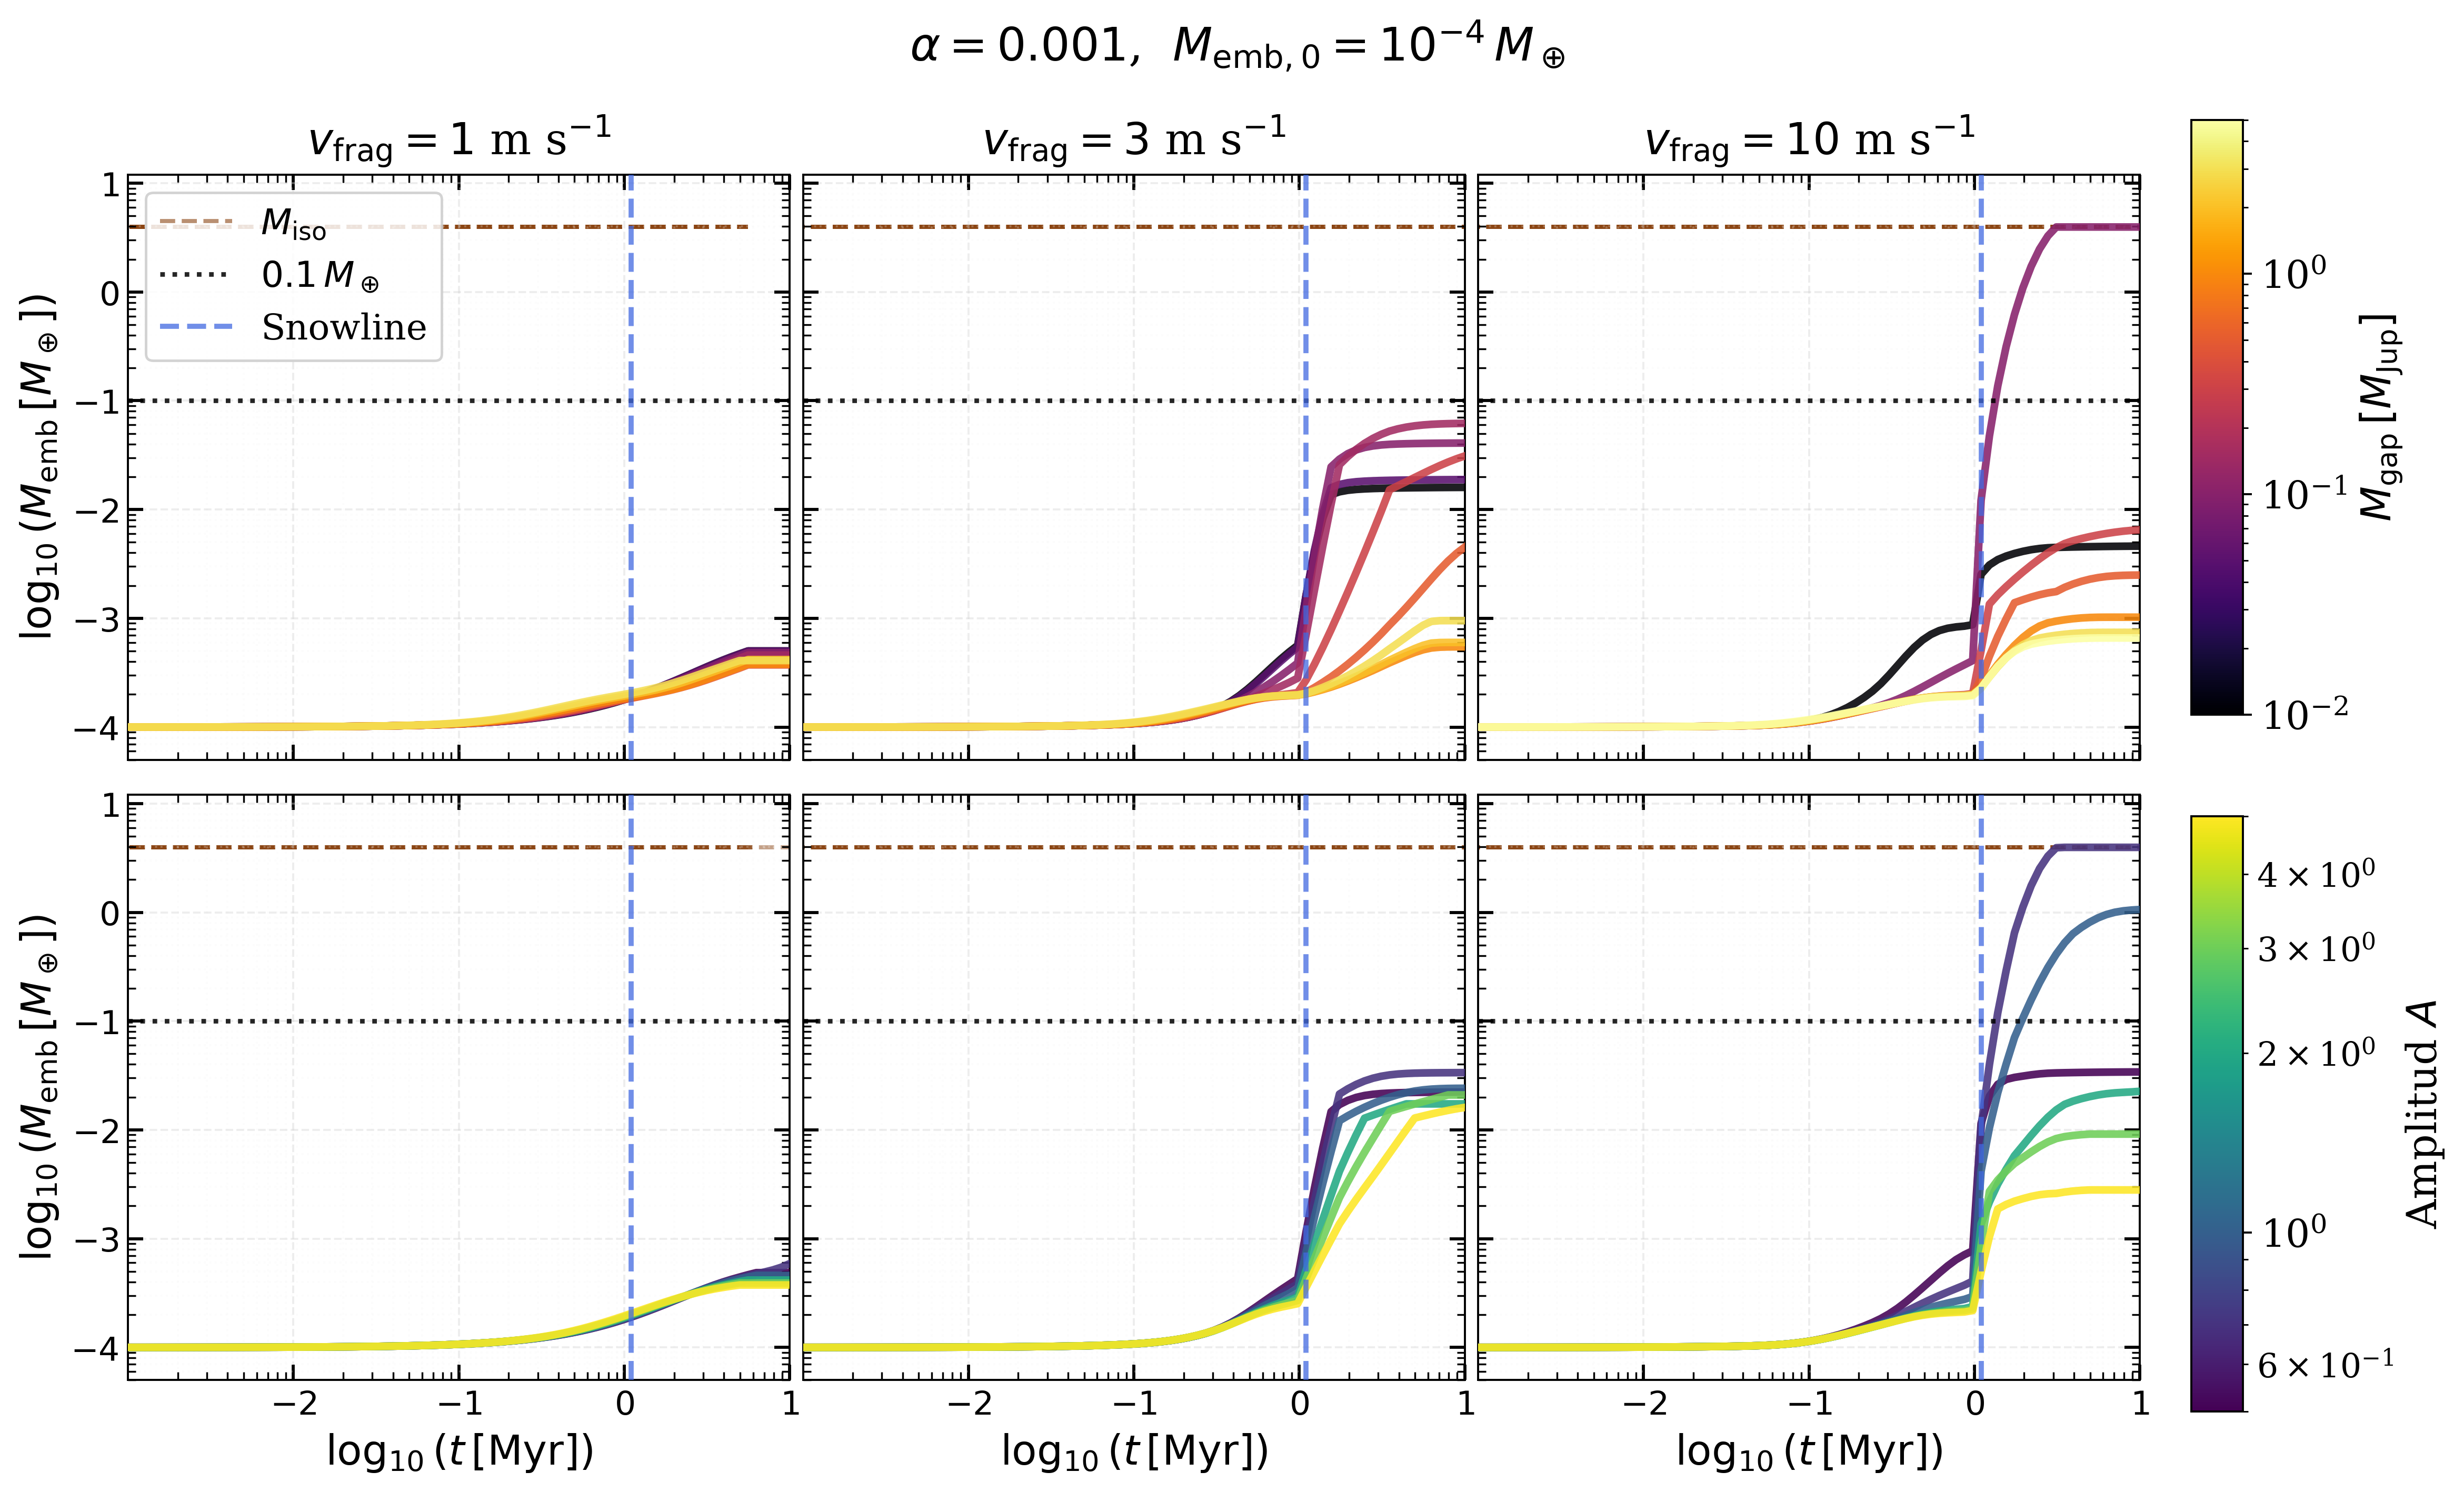
\includegraphics[width=1\textwidth]{figures/4_fig_resultados/figura_A3_gap_sinusoidal.png}
    \caption{
    Evolución temporal de la masa de un embrión situado a $1\,{\rm AU}$ para distintas velocidades de fragmentación (columnas) y configuraciones de subestructuras (filas). En la fila superior, el color representa la masa del planeta que abre un único gap; en la inferior, la amplitud de un perfil sinusoidal de viscosidad. Se adopta $\alpha=10^{-3}$ y $M_{\rm emb,0}=10^{-4}\,M_\oplus$. La línea vertical azul indica el cruce de la snowline, mientras que las líneas horizontales muestran el umbral de $0.1\,M_\oplus$ y la masa de aislamiento $M_{\rm iso}$. Se observa que el crecimiento más eficiente ocurre para valores intermedios de la intensidad de la perturbación.
}
    \label{fig:gap_sinusoidal}
\end{figure}

% =========================================================
\invisiblesubsection{Gap único}
% =========================================================

La fila superior de la Figura~\ref{fig:gap_sinusoidal} muestra la evolución temporal de la masa del embrión para un disco con un único gap localizado en $10\,{\rm AU}$, utilizando $\alpha=10^{-3}$ y una masa inicial
$M_{\rm emb,0}=10^{-4}\,M_\oplus$.

Para $v_{\rm frag}=1\,{\rm m\,s^{-1}}$, todas las trayectorias muestran un crecimiento limitado durante toda la evolución y permanecen por debajo de $10^{-3}\,M_\oplus$. Al aumentar la velocidad de fragmentación hasta $3\,{\rm m\,s^{-1}}$, las trayectorias comienzan a divergir alrededor de $t\sim10^{6}$ años, aunque ninguna supera el umbral de $0.1\,M_\oplus$.

En el caso de $v_{\rm frag}=10\,{\rm m\,s^{-1}}$, varias trayectorias experimentan un incremento pronunciado de masa después de aproximadamente $10^{6}$ años. Las mayores masas finales corresponden a valores intermedios de $M_{\rm gap}$, mientras que los gaps menos profundos y los más profundos producen masas finales considerablemente menores.

% =========================================================
\invisiblesubsection{Perfil sinusoidal}
% =========================================================

La fila inferior de la Figura~\ref{fig:gap_sinusoidal} presenta el mismo experimento utilizando un perfil sinusoidal compuesto por múltiples anillos.

El comportamiento general es similar al obtenido para el caso de un único gap. Para $v_{\rm frag}=1\,{\rm m\,s^{-1}}$, el crecimiento permanece reducido en todas las configuraciones. Al considerar $v_{\rm frag}=3\,{\rm m\,s^{-1}}$, las trayectorias comienzan a diferenciarse cerca de $1$ Myr, aunque ninguna alcanza el umbral de éxito.

Para $v_{\rm frag}=10\,{\rm m\,s^{-1}}$, la masa final depende de la amplitud de la perturbación. Las mayores masas se obtienen para amplitudes intermedias, mientras que las amplitudes más bajas y más altas producen trayectorias con crecimiento significativamente menor.

% =========================================================
\invisiblesubsection{Dependencia con la turbulencia}
% =========================================================

La Figura~\ref{fig:regimenes_alpha} muestra la evolución temporal del embrión al variar el parámetro turbulento $\alpha$, manteniendo fija la velocidad de fragmentación en $v_{\rm frag}=10\,{\rm m\,s^{-1}}$.

\begin{figure}[h!]
    \centering
    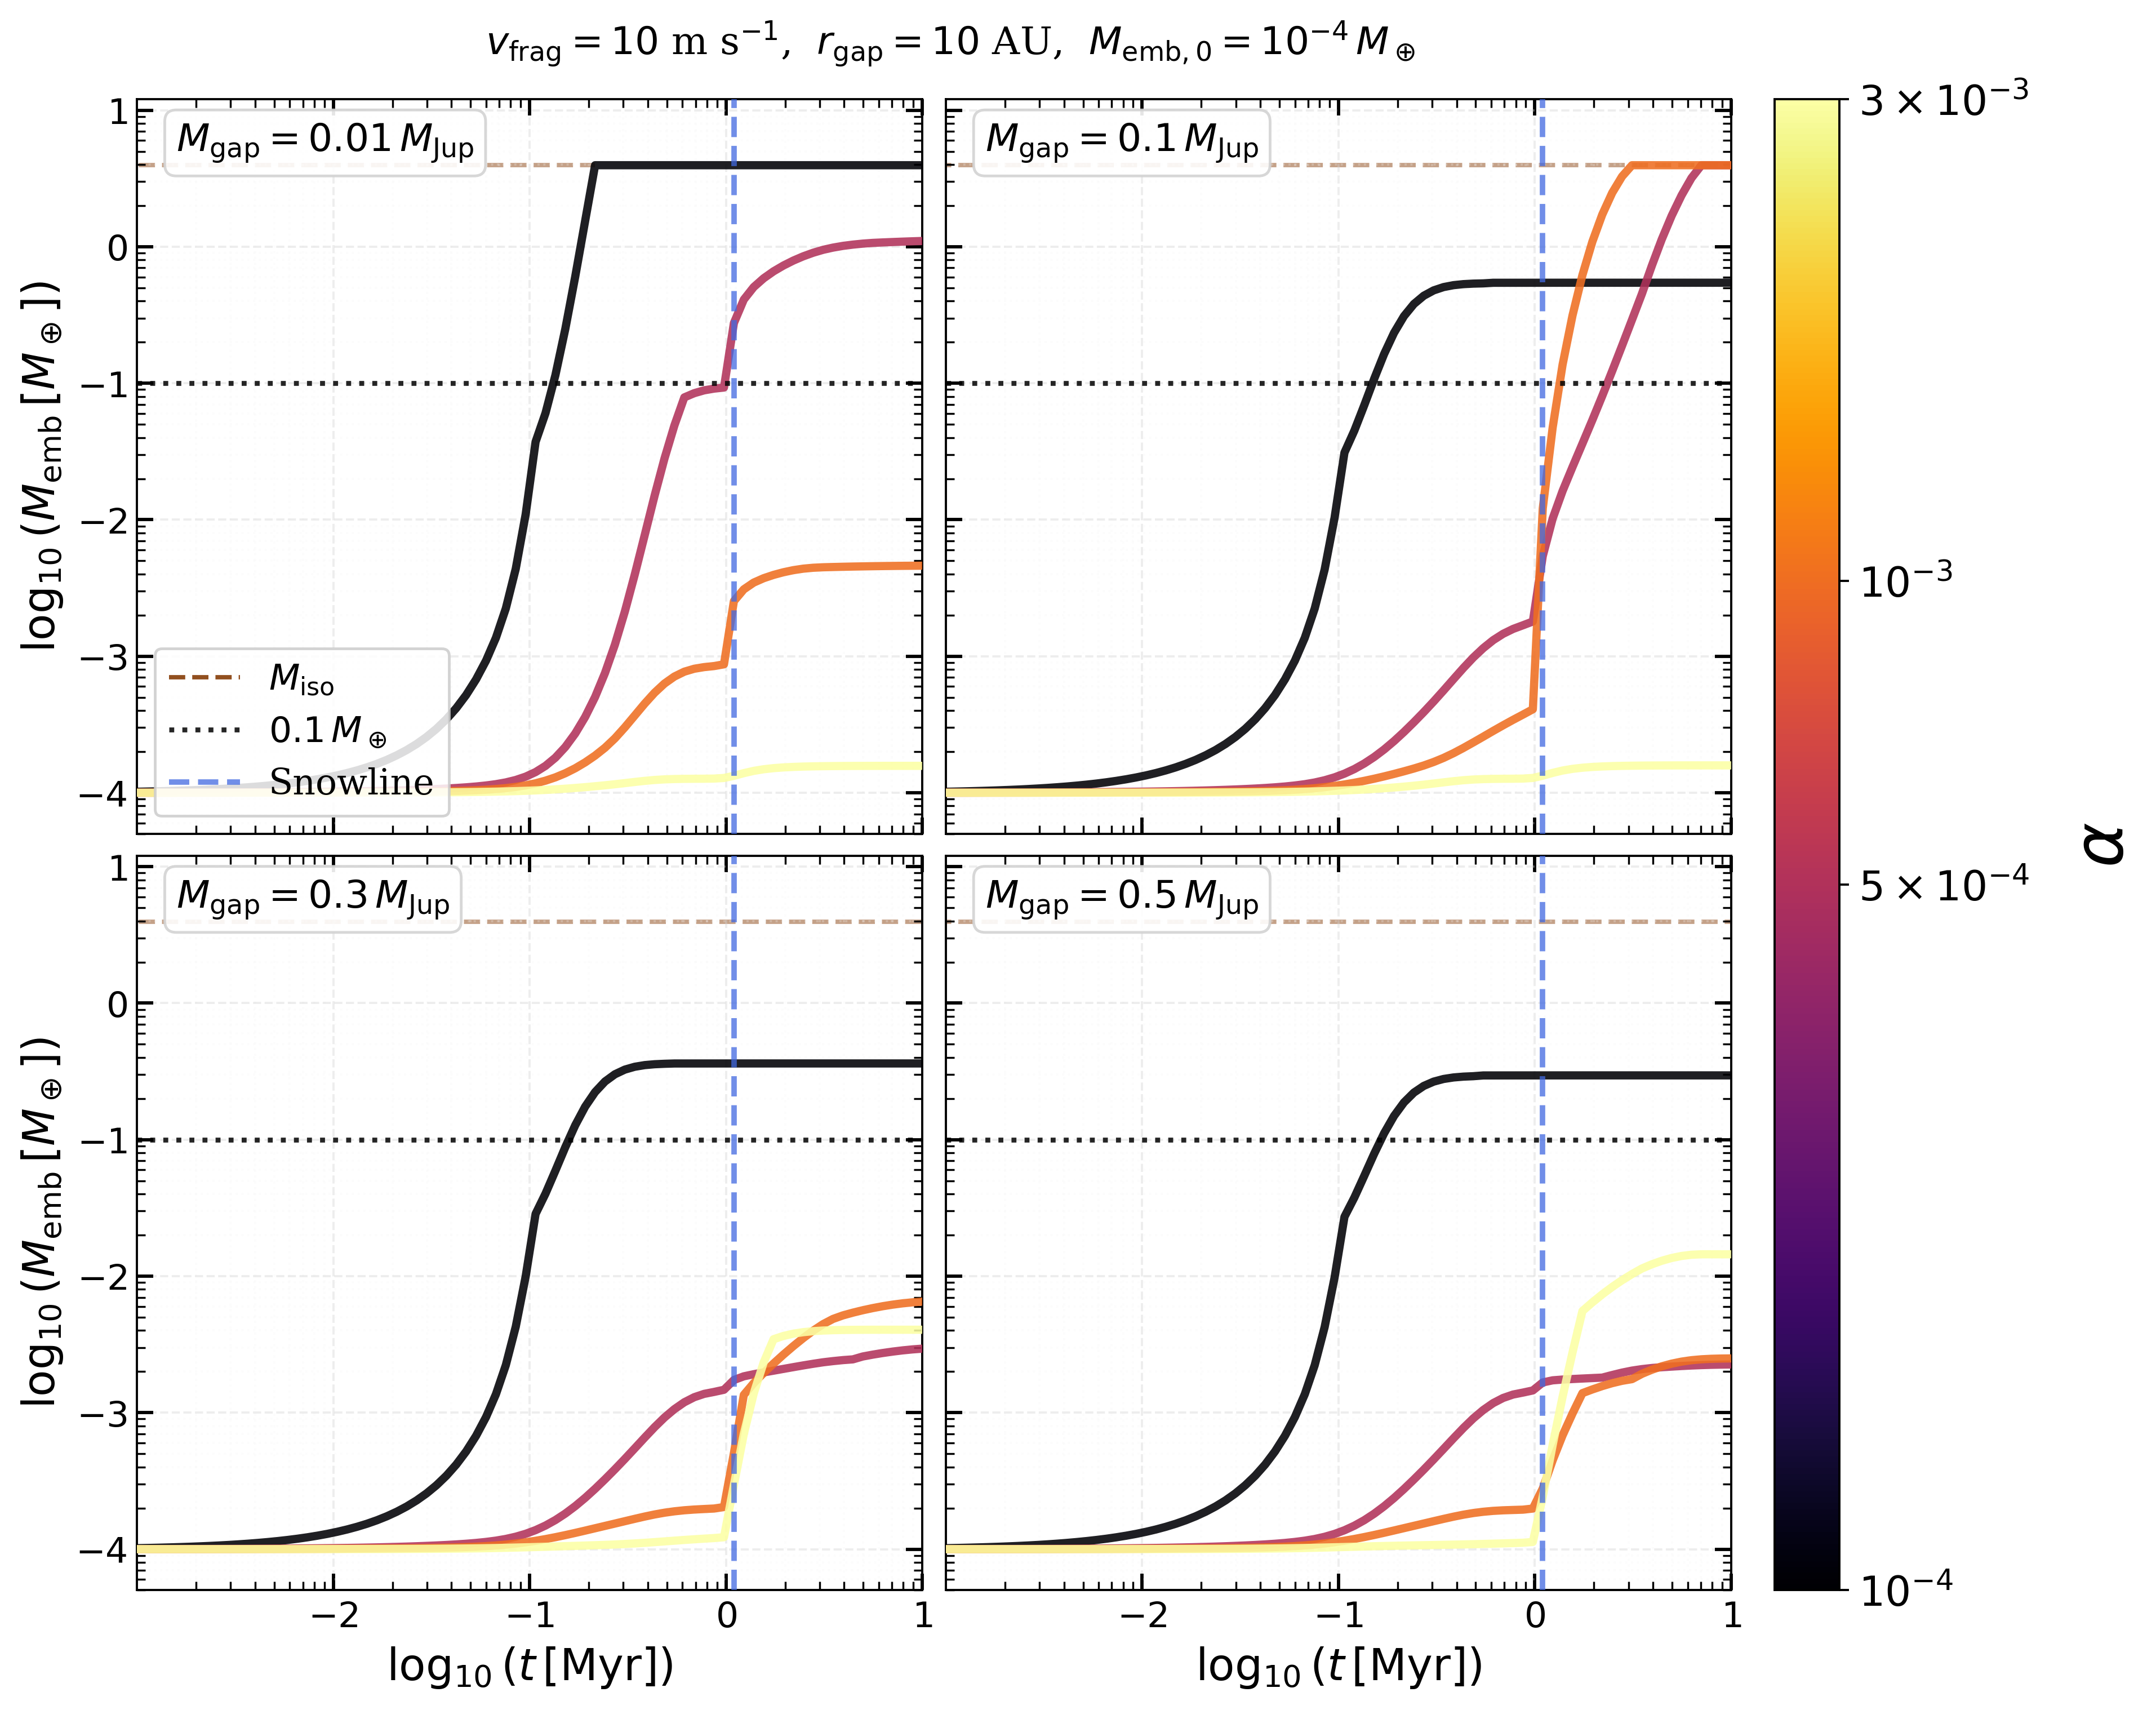
\includegraphics[width=0.8\textwidth]{figures/4_fig_resultados/figura_B_regimenes_mgap.png}
    \caption{
    Evolución temporal de la masa del embrión para distintos niveles de turbulencia. Cada panel corresponde a una masa diferente del planeta que abre el gap ($M_{\rm gap}=0.01$, $0.1$, $0.3$ y $0.5\,M_{\rm Jup}$). El color de las trayectorias representa el parámetro turbulento $\alpha$. Se mantiene fijo $v_{\rm frag}=10\,{\rm m\,s^{-1}}$, $r_{\rm gap}=10\,{\rm AU}$ y $M_{\rm emb,0}=10^{-4}\,M_\oplus$. Los ejes y las líneas de referencia son los mismos que en la Figura~\ref{fig:gap_sinusoidal}.
    }
    \label{fig:regimenes_alpha}
\end{figure}

En todas las configuraciones, las trayectorias correspondientes a los menores valores de $\alpha$ alcanzan las mayores masas finales, mientras que el crecimiento disminuye progresivamente al aumentar la turbulencia.

La dependencia con $\alpha$ varía entre paneles. En particular, el caso con $M_{\rm gap}=0.1\,M_{\rm Jup}$ presenta el mayor número de trayectorias que superan el umbral de $0.1\,M_\oplus$, mientras que para el resto de las masas del gap únicamente los valores más bajos de $\alpha$ alcanzan masas comparables.
% =========================================================
\section{Síntesis Poblacional: La Isla de Crecimiento}
\label{sec:sintesis_poblacional}
% =========================================================

Esta sección presenta un análisis global de la población final de embriones obtenida en las simulaciones, evaluando la masa final alcanzada y su composición final (fracción de agua) bajo diferentes regímenes de los parámetros explorados.

% =========================================================
\invisiblesubsection{Dinámica temporal del gap}
% =========================================================

La Figura~\ref{fig:delayed_gap} presenta la masa final del embrión en función de la fracción de agua para un escenario de alta turbulencia ($\alpha = 0.001$) con un gap ubicado en $10\,{\rm AU}$. En este panel, el tiempo en el que se forma la subestructura ($t_{\rm gap}$) se indica mediante la escala de color, mientras que la masa del planeta responsable del gap define la forma del marcador.

\begin{figure}[h!]
    \centering
    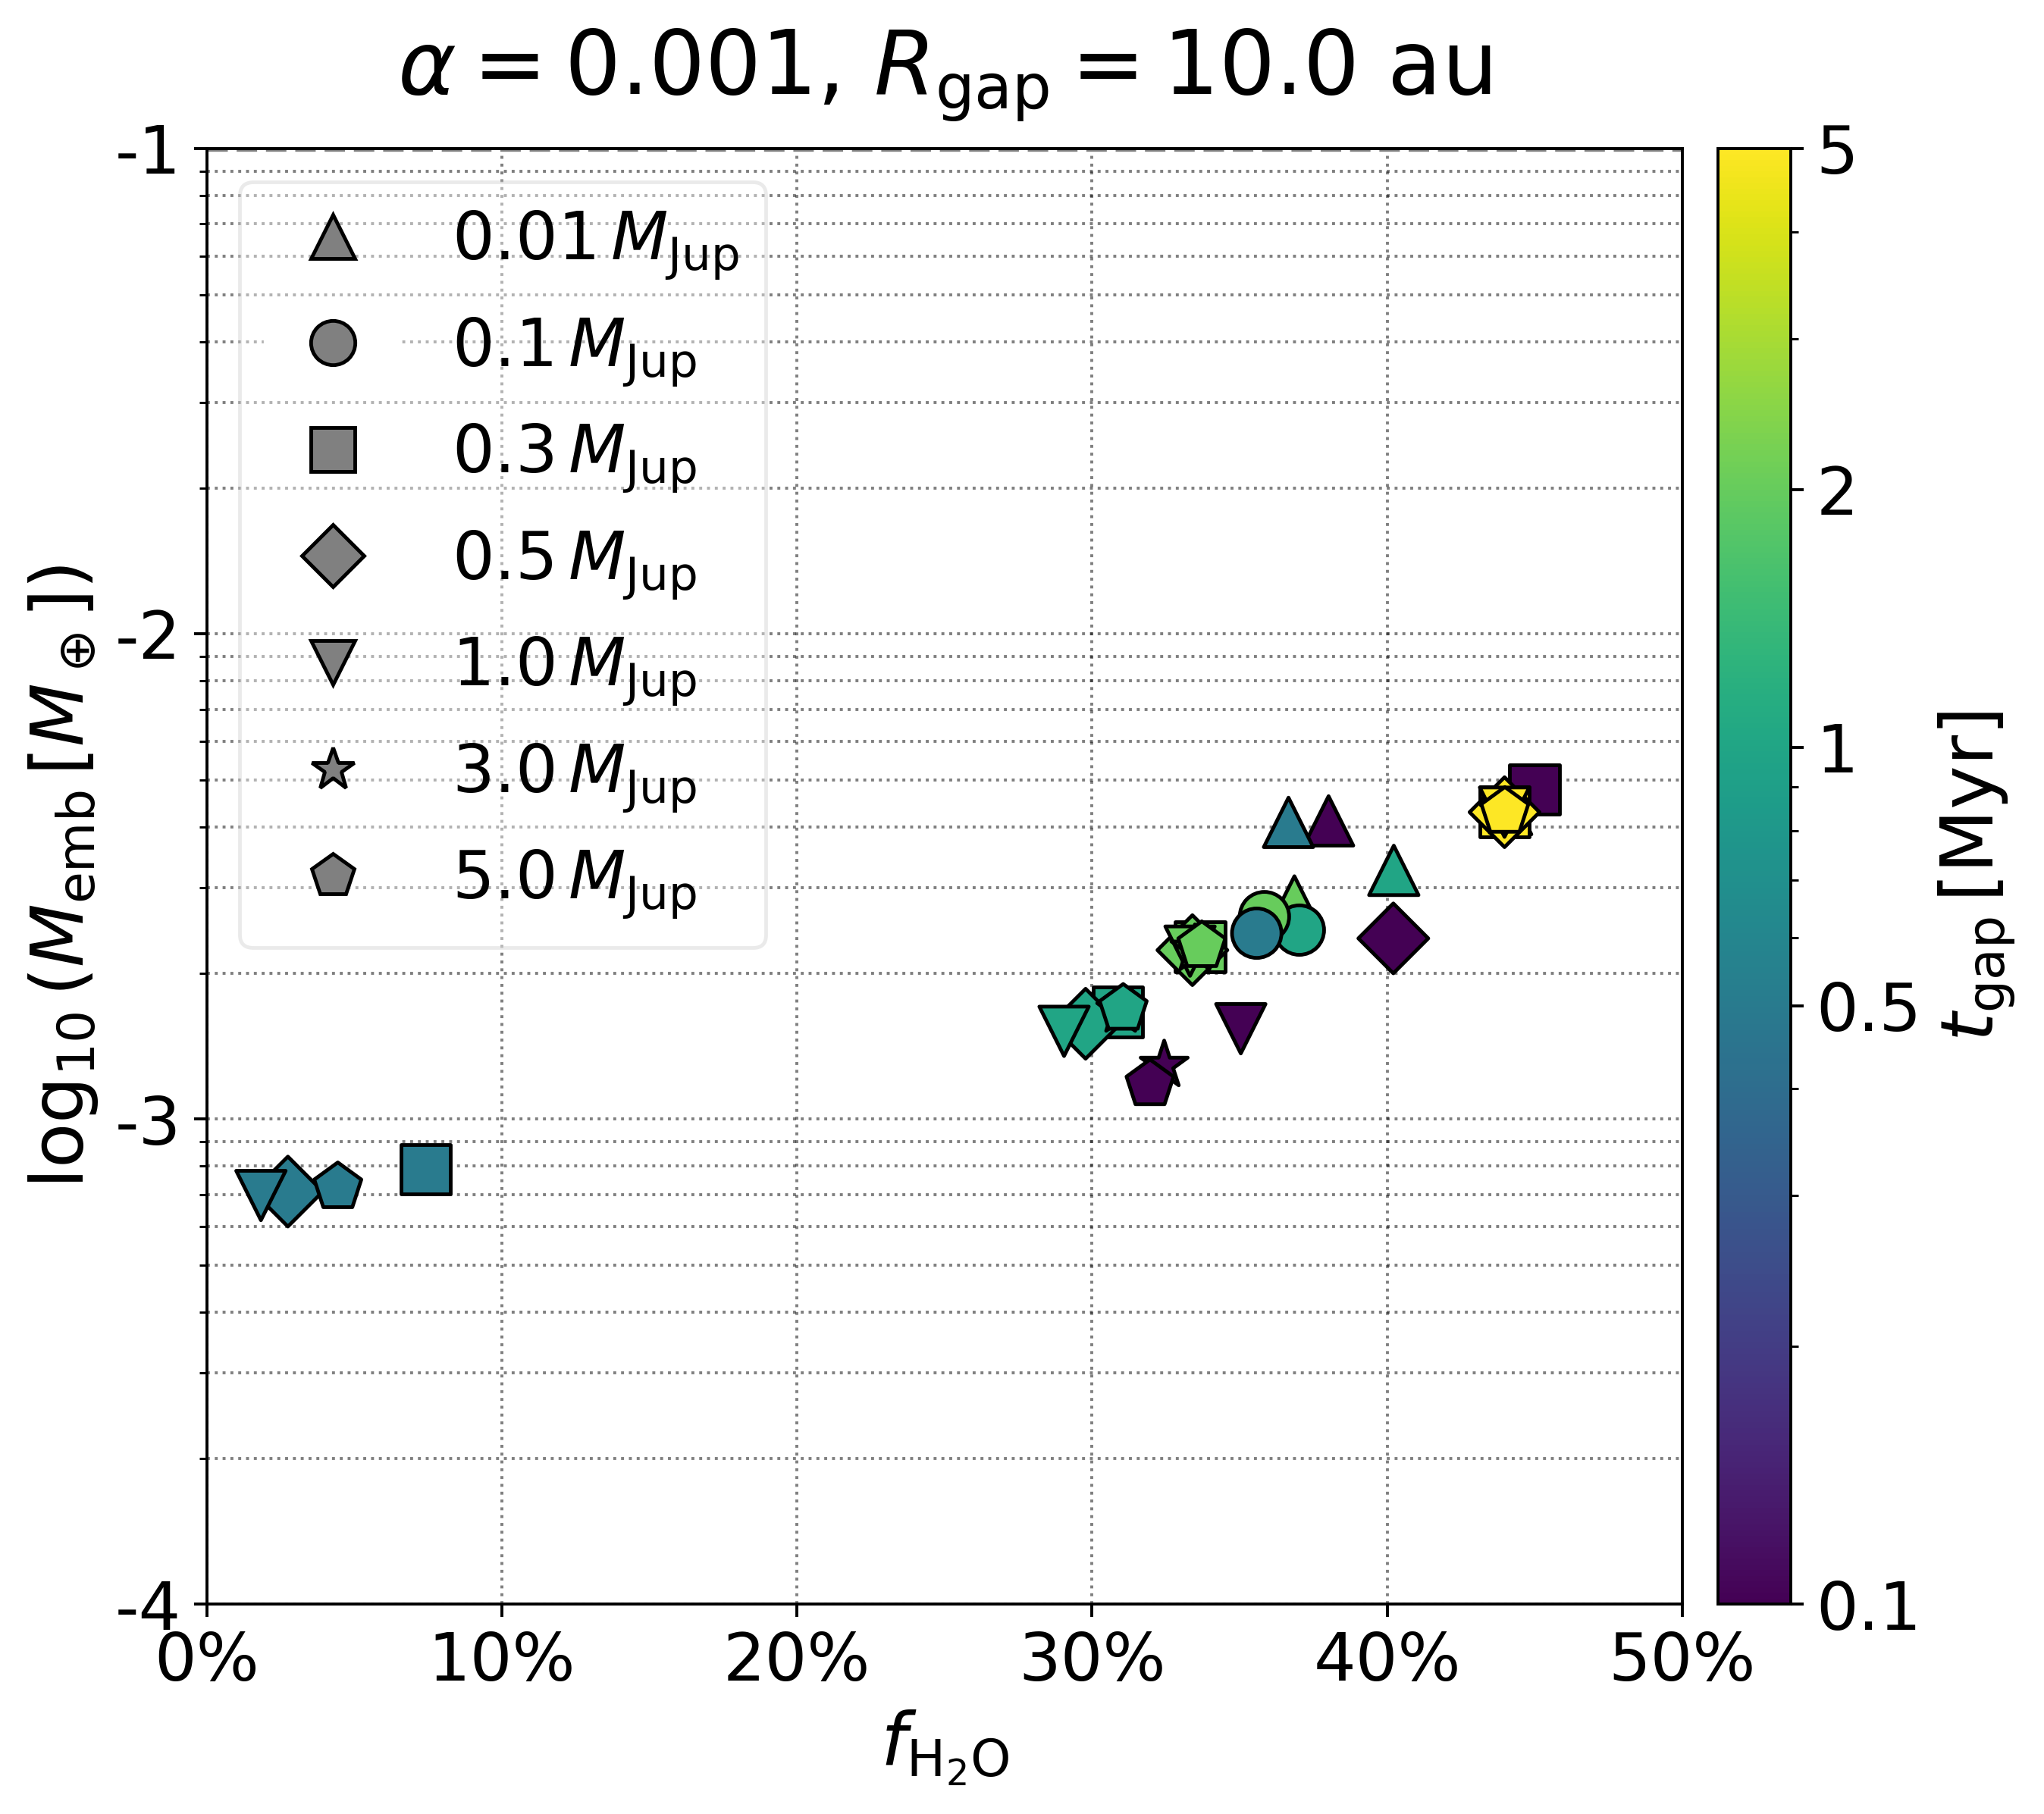
\includegraphics[width=0.75\textwidth]{figures/4.2_resultados/resultados_delayed_1x1_markers.png}
    \caption{Masa final del embrión (en escala logaritmica) versus fracción de agua (en porcentaje) para un disco con turbulencia $\alpha = 0.001$ y un gap en $r_{\rm gap}=10\,{\rm AU}$. El color de los marcadores representa el tiempo en el que se introduce el gap en la simulación ($t_{\rm gap}$) y la forma del marcador indica la masa del perturbador ($M_{\rm gap}$).}
    \label{fig:delayed_gap}
\end{figure}

Se observa una tendencia principal diagonal donde la mayoría de los casos se agrupan con fracciones de agua elevadas (entre $30\%$ y $50\%$). En este grupo convergen todas las masas de gap exploradas y una amplia variedad de tiempos de formación. Fuera de esta aglomeración, se distingue un único grupo de casos aislados en la zona de bajas fracciones de agua ($< 10\%$). Estos marcadores corresponden exclusivamente a simulaciones con un tiempo de formación de gap temprano (tonos oscuros/cian) y masas de perturbador mayores o iguales a $0.3\,M_{\rm Jup}$ (cuadrados, pentágonos, hexágonos y rombos).

% =========================================================
\invisiblesubsection{Mapa de parámetros globales}
% =========================================================

Para expandir el análisis a la grilla completa de simulaciones, la Figura~\ref{fig:mapa_global} resume los resultados variando la turbulencia, la velocidad de fragmentación y las características espaciales de la subestructura. 

\begin{figure}[h!]
    \centering
    
\includegraphics[width=\textwidth]{figures/4.2_resultados/resultados_bubble.png} 
    \caption{Mapa de resultados que sintetiza la población final. Las columnas varían la turbulencia $\alpha$ y las filas la velocidad de fragmentación $v_{\rm frag}$. El tamaño del círculo representa una aproximación de la masa final y el color indica la fracción de agua. Los marcadores circulares indican casos exitosos ($\ge 0.1\,M_\oplus$), mientras que los triángulos invertidos representan fracasos.}
    \label{fig:mapa_global}
\end{figure}

El panel muestra que el mayor número de casos exitosos (marcadores circulares) ocurre para bajas turbulencias ($\alpha=10^{-4}$) y altas velocidades de fragmentación ($v_{\rm frag}=10\,{\rm m\,s^{-1}}$). Particularmente para este último valor de $v_{\rm frag}$ (fila inferior), se aprecia una franja horizontal de éxito sostenido concentrada en profundidades de gap entre $0.05$ y $0.1\,M_{\rm Jup}$. Esta banda mantiene la formación de embriones masivos, con altas fracciones de agua (tonos naranjas/amarillos), incluso al aumentar la turbulencia hacia las columnas de la derecha. Las configuraciones con gaps más profundos o velocidades de fragmentación menores presentan predominantemente marcadores de fracaso.

% =========================================================
\invisiblesubsection{Distribución composicional}
% =========================================================

La Figura~\ref{fig:facet_lineal} examina explícitamente la relación entre la masa final y la composición para las distintas arquitecturas del disco (gap único y perfil sinusoidal). 

\begin{figure}[h!]
    \centering
    
\includegraphics[width=\textwidth]{figures/4.2_resultados/figura_C_facet_combinado_lineal.png}
    \caption{Masa final del embrión versus fracción de agua (escala lineal) para distintos valores de turbulencia (columnas). La fila superior corresponde a un gap único y la inferior a un perfil sinusoidal. El color indica la velocidad de fragmentación.}
    \label{fig:facet_lineal}
\end{figure}

Al observar la secuencia de izquierda a derecha (incremento de $\alpha$), la distribución de la población muestra un colapso generalizado hacia el extremo derecho de los paneles. Para $\alpha \ge 5\times10^{-4}$, la inmensa mayoría de los embriones que superan el umbral de masa exhiben fracciones de agua cercanas al $50\%$.

Sin embargo, en la primera columna correspondiente a la turbulencia más baja ($\alpha=10^{-4}$), la distribución es notablemente diferente. Además de los casos ricos en agua, se acumula un conjunto visible de simulaciones que alcanzan masas por encima de $0.1\,M_\oplus$ manteniendo fracciones de agua sumamente bajas (cercanas al margen izquierdo del panel).

Para visualizar con mayor precisión esta subpoblación específica, la Figura~\ref{fig:facet_log} presenta la misma distribución para $\alpha=10^{-4}$, restringiendo el eje horizontal al rango de $0\%$ a $10\%$ mediante una escala logarítmica.

\begin{figure}[h!]
    \centering
    
\includegraphics[width=0.85\textwidth]{figures/4.2_resultados/figura_C_facet_combinado_log_10pct.png}
    \caption{Detalle de la masa final versus fracción de agua en escala logarítmica para $\alpha=10^{-4}$, enfocado en el rango de $0\%$ a $10\%$ de composición de agua. El sombreado destaca distintas zonas de acumulación en los escenarios de gap único (arriba) y perfil sinusoidal (abajo).}
    \label{fig:facet_log}
\end{figure}

El gráfico evidencia claramente la existencia de una agrupación de planetas masivos y predominantemente secos, los cuales exhiben fracciones de agua de entre $0\%$ y $2\%$. Esta subpoblación se distingue nítidamente tanto en la configuración de gap único como en la sinusoidal bajo este nivel específico de turbulencia.